\documentclass[b5paper,10pt]{jsarticle}

\usepackage{bxpapersize}
% コード
\usepackage{listings,jvlisting}
\lstset{
basicstyle={\ttfamily},
identifierstyle={\small},
commentstyle={\small\ttfamily \color[rgb]{0,0.5,0}},
keywordstyle={\small\bfseries \color[rgb]{0,0,0.8}},
ndkeywordstyle={\small},
stringstyle={\small\ttfamily \color[rgb]{0,0,1}},
frame={tb},
breaklines=true,
columns=[l]{fullflexible},
numbers=left,
xrightmargin=0zw,
xleftmargin=3zw,
numberstyle={\scriptsize},
stepnumber=1,
numbersep=1zw,
lineskip=-0.5ex
}
\renewcommand{\lstlistingname}{プログラム}
%フォント
\usepackage{lmodern}
%脚注
\usepackage[stable]{footmisc}
%特殊文字
\usepackage{otf}
\usepackage{mathrsfs}
%ルビ
\usepackage{pxrubrica}
% 数式
\usepackage{amsmath,amsfonts,amssymb,amsthm}
\usepackage{bm}
\usepackage{bbm}
\usepackage{mathcomp}
\usepackage{braket,physics}
\usepackage{gensymb}
\usepackage[legacycolonsymbols]{mathtools}

% 画像
\usepackage{color}
\usepackage{float}
\usepackage[dvipdfmx]{graphicx}
% TikZ
\usepackage{tikz}
\usetikzlibrary{intersections, calc, arrows.meta}
\usetikzlibrary{3d}
\usepackage{pgfplots}
\pgfplotsset{compat=1.18}
\usepackage{subcaption}
%表
\usepackage{booktabs}
%箇条書き
\usepackage{enumerate}
% 囲み
\usepackage{ascmac}
\usepackage{fancybox}
\usepackage{tcolorbox}
%footer
\usepackage{fancyhdr}
\pagestyle{fancy}

\usepackage{tikz}
\usetikzlibrary{quantikz} % 量子回路専用のライブラリ
%caption
\usepackage{caption}
%hyperlink
\usepackage[dvipdfmx]{hyperref}
\usepackage{pxjahyper}
\hypersetup{% hyperrefオプションリスト
setpagesize=false,
 bookmarksnumbered=true,%
 bookmarksopen=true,%
 colorlinks=true,%
 linkcolor=blue,
 citecolor=red,
}
\DeclareMathOperator*{\argmax}{arg\,max}

\newtcolorbox{examplebox}[1][]{
    colback=blue!5,
    colframe=blue!50!black,
    title=例,
    fonttitle=\bfseries,
    #1
  }

\begin{document}
\fancyfoot[L]{東京大学 第99回 五月祭}
\fancyfoot[R]{応用物理学系 工学博覧会}
%ここまでは原則として変えない 


\quad

\hrule\vskip.5mm\hrule
\section{ベイズ回帰(ボードゲーム班)}
\hrule \vskip.5mm\hrule
\vspace{1em}
\subsection{はじめに}
(この記事の執筆時点で, 企画の詳細が定まっていないため, ボードゲーム班の企画とどの程度関連があるのかは分かりませんが, ご了承ください. )\\
ベイズ的な考え方はニューラルネットワークなどの機械学習の分野でもよく用いられており, ベイジアンニューラルネットワーク (BNN) などが知られています. 
ここでは BNN 自体は扱いませんが, 直感的に理解しやすい回帰という問題設定において, ベイズ的な考え方と, それとよく対比される頻度論的 (frequentist)な考え方を比較して, ベイズの有用性を探ります. \\
他の記事は難しそうなのですが, この記事は高校生でも理解できる説明を目指します. 
\subsection{回帰}
まず, 回帰について説明します. ここで扱う回帰とは, 二つのデータの組 $(x_i, y_i)$ が与えられたときに, それらの関係を推定する問題です(なお, 一般的には「回帰」はもっと広い問題設定ですが, ここではその特別な場合を扱います). 
さっそく例を見てみましょう. 
\begin{examplebox}
ある現象を観測して, 次のようなデータが得られたとします. 
\begin{figure}[H]
    \centering
    \begin{minipage}[t]{0.45\textwidth}
      \centering
      \captionof{table}{データ}
      \label{tab:data}
      \begin{tabular}{c|c}
        $x$ & $y$ \\
        \hline
        1.47 & 0.99 \\
        0.47 & 0.53 \\
        -1.78 & -0.82 \\
        1.53 & 0.69 \\
        -0.41 & -0.36 \\
      \end{tabular}
    \end{minipage}
    \hfill
    \begin{minipage}[t]{0.50\textwidth}
      \centering
      \captionof{figure}{データのプロット}
      \label{fig:data-plot}
      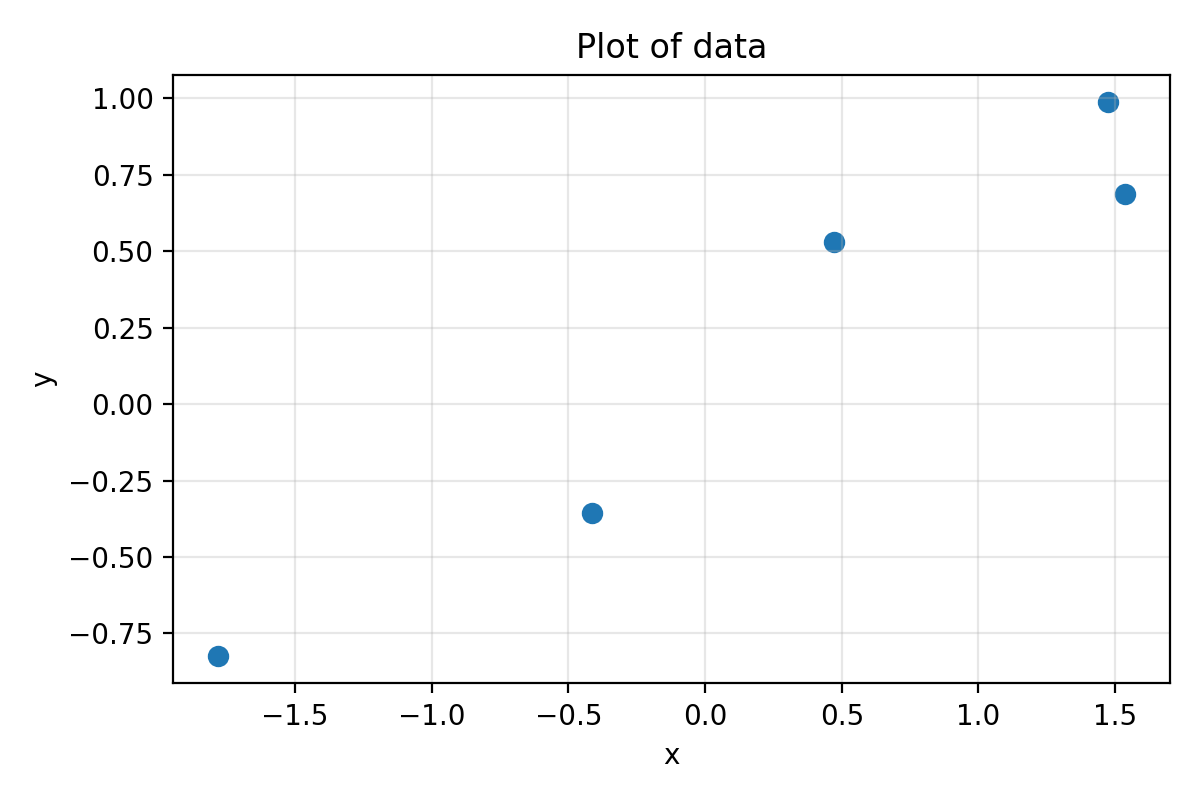
\includegraphics[width=\linewidth]{images/figure1.png}
    \end{minipage}
\end{figure}
ここで, この現象は $y = w_0 + w_1 x + w_2 x^2 + w_3 x^3$ というモデルでそれなりによく近似できると仮定します. どのようにして $x$ と $y$ の関係性を推定すれば良いでしょうか？
\end{examplebox}
ここでいう「関係性」とは, パラメータ $w_0, w_1, w_2, w_3$ のことだと思っていただいて構いません. 実際, もしこれらを知ることができたら, この現象は十分解明できたと言えるでしょう. 
\subsection{頻度論的な考え方}
頻度論という言葉は馴染みがないかもしれませんが, 高校や大学でやるような, 最小二乗法で最も近似できる曲線を求めることを考えます. 先ほどの問題に最小二乗法を適用してみましょう. \\
$x = x_i$ に対して, モデルの予測値は $\hat{y}_i = w_0 + w_1 x_i + w_2 x_i^2 + w_3 x_i^3$ となります. この予測値と実際のデータ $y_i$ の誤差は $y_i - \hat{y}_i$ となります. この誤差の二乗の平均を最小化するような $w_0, w_1, w_2, w_3$ を求めることが目標です. \\
式で書くと, 
\begin{align*}
    E(w_0, w_1, w_2, w_3) := \frac{1}{5}\sum_{i=1}^5 (y_i - \hat{y}_i)^2 = \frac{1}{5}\sum_{i=1}^5 (y_i - (w_0 + w_1 x_i + w_2 x_i^2 + w_3 x_i^3))^2
\end{align*}
と定義した誤差関数 $E$ について, $E$ を最小化するような $w_0, w_1, w_2, w_3$ を求めれば良いです. これらは, 各 $w_i$ について偏微分するなどして求めることができます. コンピュータによる計算の結果は以下のようになります. \\
$w_0 = 0.0790, w_1 = 1.09, w_2 = -0.0618, w_3 = -0.218$ \\
これをプロットすると次のようになります. 
\begin{figure}[H]
  \centering
  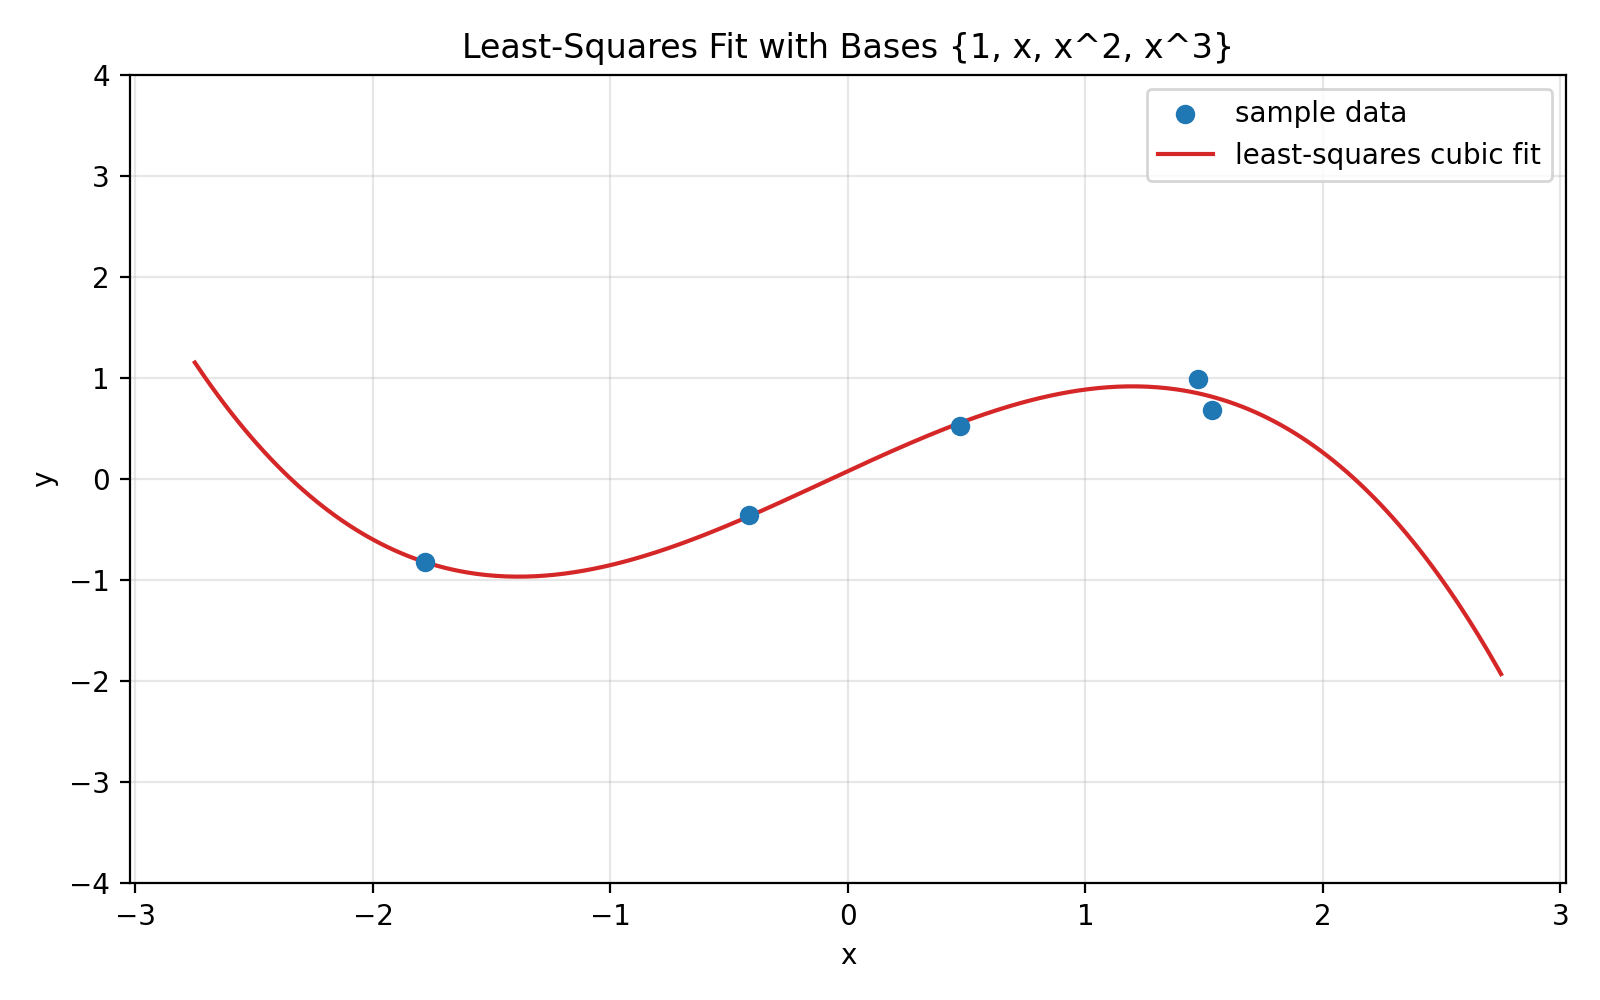
\includegraphics[width=0.7\textwidth]{images/frequentist1_fit.png}
  \caption{頻度論的な考え方による近似}
  \label{fig:frequentist1}
\end{figure}
見ての通り, 直感的にはよく近似できているように見えます. ただし, 一つ問題があります. たった 5 つのデータで推定した結果がどのくらい信用できるでしょうか？ もしたまたま, 本来なら外れ値であるはずのデータがここに入っていたらどうでしょうか？ 
まだこの現象をきちんと理解したと言い切るには早い気がします. 
\subsection{ベイズ的な考え方}
前置きが長くなりましたが, ベイズ的な考え方を用いてこの問題を解いてみましょう. 頻度論的な考え方の欠点は, データが少ないにも関わらず関係性($w_i$ というパラメータ)を一つだけ推定してしまい, その結果がどれだけ信頼できるかわからないことでした. これに対して, ベイズ線形回帰は各パラメータを確率分布として推定することでこの問題に対処します. 
具体的には以下の流れで行います. 
\begin{enumerate}
    \item パラメータ $w_0, w_1, w_2, w_3$ の事前分布と, データ $y_i$ の分布を仮定する.
    \item ベイズの定理を用いて, 与えられたデータからパラメータ $w_0, w_1, w_2, w_3$ の事後分布を計算する. 
    \item 事後分布から, 予測分布を計算する. 
\end{enumerate}
\subsubsection{事前分布の仮定}
まず, パラメータ $w_0, w_1, w_2, w_3$ の事前分布を与えます. ここでは, はじめ各 $w_i$ が独立に平均 $0$, 分散$\sigma_w^2$ のガウス分布(正規分布)に従っていると仮定します. 
一方, データ $y_i$ は平均 $w_0 + w_1 x_i + w_2 x_i^2 + w_3 x_i^3$, 分散$\sigma_y^2$ のガウス分布に従っていると仮定します.  すなわち, 
\begin{align}
    p(w_0, w_1, w_2, w_3) &= \prod_{i=0}^3 \mathcal{N}(w_i | 0, \sigma_w^2) \label{eq:prior} \\
    p(y_i | x_i, w_0, w_1, w_2, w_3) &= \mathcal{N}(y_i | w_0 + w_1 x_i + w_2 x_i^2 + w_3 x_i^3, \sigma_y^2) \label{eq:likelihood}
\end{align}
ここで, $\mathcal{N}(x | \mu, \sigma^2)$ は平均 $\mu$, 分散 $\sigma^2$ のガウス分布の確率密度関数を表します. 具体的には, \\
\begin{align*}
    \mathcal{N}(x | \mu, \sigma^2) = \frac{1}{\sqrt{2\pi\sigma^2}} \exp\left(-\frac{(x - \mu)^2}{2\sigma^2}\right)
\end{align*}
です. \\
なお, ここでの二つの分散は勝手に仮定したもので, 人間が適当に決めます. \\
この段階ではまだデータを使っておらず, パラメータの分布は不正確です. ここからデータを用いてパラメータの分布をもっともらしいものに近づけていきます. そうすることで, より確からしい関係性を推定することができます. 
\subsubsection{事後分布の計算}
次に, 与えられたデータとベイズの定理から, $w_i$ の事後分布を計算します. 以下, 表記の簡略化のために, $w_0, w_1, w_2, w_3$ をまとめて $\bm{w}$ と書き, データ $(x_i, y_i)$ をまとめて $\mathcal{D}$ と書きます. \\
ベイズの定理より, 
\begin{align}
    p(\bm{w} | \mathcal{D}) = \frac{p(\mathcal{D} | \bm{w}) p(\bm{w})}{p(\mathcal{D})}
\end{align}
これを計算していきます. ここで, \eqref{eq:prior}と\eqref{eq:likelihood}より, 
\begin{align}
    p(\mathcal{D} | \bm{w}) &= \prod_{i=1}^5 \mathcal{N}(y_i | w_0 + w_1 x_i + w_2 x_i^2 + w_3 x_i^3, \sigma_y^2) \\
    p(\bm{w}) &= \prod_{i=0}^3 \mathcal{N}(w_i | 0, \sigma_w^2)
\end{align}
なので(以下, 途中で出てくる $\bm{w}$ に関係ない定数は重要でないので \text{const} と書きます), 
\begin{align}
    p(\bm{w} | \mathcal{D}) &= \frac{1}{p(\mathcal{D})} \left(\prod_{i=1}^5 \frac{1}{\sqrt{2\pi\sigma_y^2}} \exp\left(-\frac{(y_i - (\sum_{j=0}^3 w_j x_i^j))^2}{2\sigma_y^2}\right)\right) \prod_{i=0}^3 \frac{1}{\sqrt{2\pi\sigma_w^2}} \exp\left(-\frac{w_i^2}{2\sigma_w^2}\right) \\
    &= \text{const} \times \prod_{i=1}^5 \exp\left(-\frac{(y_i - (\sum_{j=0}^3 w_j x_i^j))^2}{2\sigma_y^2}\right) \prod_{i=0}^3 \exp\left(-\frac{w_i^2}{2\sigma_w^2}\right) \\
    &= \text{const} \times \exp\left(-\frac{1}{2\sigma_y^2} \sum_{i=1}^5 (y_i - (\sum_{j=0}^3 w_j x_i^j))^2 - \frac{1}{2\sigma_w^2} \sum_{i=0}^3 w_i^2\right) \\
    &= \text{const} \times \exp\left(-\sum_{i=0}^3 \left(\left(\frac{1}{2\sigma_w^2} + \frac{1}{2\sigma_y^2}\sum_{j=1}^5 x_j^{2i} \right) w_i^2 - \frac{1}{\sigma_y^2} \sum_{j=1}^5 y_j x_j^i w_i\right)\right) \\
    &= \text{const} \times \prod_{i=0}^3 \exp\left(-\cfrac{1}{2\left(\cfrac{1}{\cfrac{1}{\sigma_w^2} + \cfrac{1}{\sigma_y^2}\sum_{j=0}^5 x_j^{2i}}\right)} \left(w_i - \cfrac{\sum_{j=0}^{5} y_j x_j^{i}}{\cfrac{\sigma_y^2}{\sigma_w^2} + \sum_{j=0}^5 x_j^{2i}} \right)^2\right) \label{eq:posterior}
\end{align}
さて, 計算が長くなってしまいましたが, \eqref{eq:posterior}式は, 定数を考えなければガウス分布の積のような形をしています. 実際, 定数部分 \text{const} は, 確率密度関数を積分したときに 1 になることを保証する規格化定数で, 
結局 \eqref{eq:posterior}式は, 
\begin{align}
    p(\bm{w} | \mathcal{D}) = \prod_{i=0}^3 \mathcal{N}(w_i | \mu_{w_i}, \sigma_{w_i}^2)
\end{align}
と書けます. 
ここで, 
\begin{align}
    \mu_{w_i} &= \cfrac{\sum_{j=0}^{5} y_j x_j^{i}}{\cfrac{\sigma_y^2}{\sigma_w^2} + \sum_{j=0}^5 x_j^{2i}} \label {eq:mu_{w_i}} \\ 
    \sigma_{w_i}^2 &= \cfrac{1}{\cfrac{1}{\sigma_w^2} + \cfrac{1}{\sigma_y^2}\sum_{j=0}^5 x_j^{2i}} \label {eq:sigma_{w_i}^2}
\end{align}
としました. \\
このセクションの結果をまとめると, データ $\mathcal{D}$ によって, パラメータ $\bm{w}$ の分布を更新することができて, 
具体的には $w_i$ はそれぞれ \eqref{eq:mu_{w_i}} と \eqref{eq:sigma_{w_i}^2} から定まるガウス分布 $\mathcal{N}(\mu_{w_i}, \sigma_{w_i}^2)$ に従うと考えることができます. 
これは先ほどの頻度論的な考え方(最小二乗法)とは明らかに違いますね. 最小二乗法では $\bm{w}$ の値は一つに決まりましたが, ここではどの値をとるか定まっておらず確率的です. 
\subsubsection{予測分布の計算}
最後に, 更新したパラメータ(の分布)を使って, $x_i$ と $y_i$ の関係性を推定することを考えましょう. もともとこれが目的でした. そのために, 新しく $x_k$ が与えられたときに, 
それに対応する $y_k$ がどうなるかを考えます. 素直に以下の式で計算すると少し大変です. 
\begin{align}
    p(y_k | x_k, \mathcal{D}) &= \int p(y_k | x_k, \bm{w}) p(\bm{w} | \mathcal{D}) d\bm{w} 
\end{align}
これを計算せず, ガウス分布の再生性という性質を用いると,  \eqref{eq:likelihood} と \eqref{eq:posterior} より(詳細は省きますが), 
\begin{align}
    p(y_k | x_k, \mathcal{D}) = \mathcal{N}\left(y_k \mid \sum_{i=0}^3 \mu_{w_i} x_k^i, \sum_{i=0}^3 \sigma_{w_i}^2 x_k^{2i} + \sigma_y^2\right)
\end{align}
となります. これも最小二乗法の結果と違うことがわかります. 最小二乗法では, $y_k = \sum_{i=0}^3 w_i x_k^i$ と決定的に値が決まりますが, ここではやはり確率的に $y_k$ の値を推定しています. 

\end{document}